\documentclass{article}
\usepackage{tikz}
\usetikzlibrary{shapes,decorations,shadows}
\usetikzlibrary{decorations.pathmorphing}
\usetikzlibrary{decorations.shapes}
\usepackage{verbatim}

\begin{comment}
:Title: TikZ and PGF version 2.00
:slug: pgf-version-2
:Tags: PGF 2.0, Manual
:Grid: 3x3


PGF version 2.0 was released on 2008-02-20 after a few months of hectic activity in CVS and on the `pgf-users`_ mailing list. The release is packed with new features
and improvements. 


Revamped system for handling options and styles
-----------------------------------------------

PGF now ships with the new ``pgfkeys`` package. The package provides a powerful key-value management mechanism


Decorations
-----------

Decorations are a new and powerful way of decorating and morphing paths. They are similar to the "snakes" from previous versions of PGF, but much more powerful and general. Here are a few highlights:

- Arbitrary paths can be decorated, including curves and nodes
- Shapes can be used as decorations
- Decorations can be nested


Here are a few examples:

.. figure:: #pgf2001.png

.. sourcecode:: latex

    % Decorating a node shape
    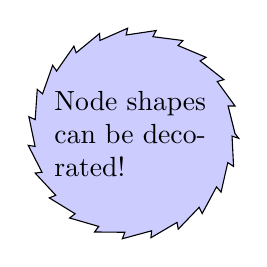
\begin{tikzpicture}
        \node [text width=2cm, decorate, decoration=saw, fill=blue!20,draw,circle]
            {Node shapes can be decorated!};
    \end{tikzpicture}
    
.. sourcecode:: latex

    % Text decorations
    \usetikzlibrary{decorations.text}
    ...
    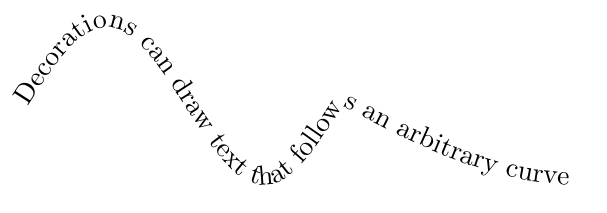
\begin{tikzpicture}
        \path [decorate,decoration={text along path,
            text={Decorations can draw text that follows an arbitrary curve}}]
            (0,0) sin (1,1) cos (2,0) sin (3,-1) cos (4,0) sin (7,-1);
    \end{tikzpicture}


.. sourcecode:: latex

    % Footprints!
    \usetikzlibrary{decorations.footprints}
    ...
    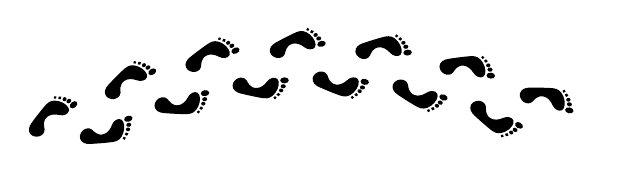
\begin{tikzpicture}[decoration={footprints,foot length=20pt}]
        \fill [decorate] (0,0) to[bend left] (7,0);
    \end{tikzpicture}




New libraries
-------------

Shadow
~~~~~~


:Source: The PGF and TikZ manual

.. _pgf-users: http://www.nabble.com/pgf-users-f3583.html
.. _changelog: ftp://cam.ctan.org/tex-archive/graphics/pgf/base/doc/generic/pgf/ChangeLog

\end{comment}


\usetikzlibrary{decorations.text}
\usetikzlibrary{decorations.footprints}
\usetikzlibrary{decorations.fractals}

\begin{document}


\tikzset{paint/.style={ draw=#1!50!black, fill=#1!50 },
    decorate with/.style=
    {decorate,decoration={shape backgrounds,shape=#1,shape size=2mm}}}

\begin{tikzpicture}
\node [text width=2cm, decorate, decoration=saw, fill=blue!20,draw,circle] 
    {Node shapes can be decorated!};
\begin{scope}[xshift=2cm]
    \path [decorate,decoration={text along path,
            text={Decorations can draw text that follows an arbitrary curve}}]
            (0,0) sin (1,1) cos (2,0) sin (3,-1) cos (4,0) sin (7,-1);
\end{scope}
%
\begin{scope}[xshift=-1.5cm,yshift=-4cm]
    \draw [decorate with=dart, paint=red] (0,1.5) to[bend left] (3,1.5);
    \draw [decorate with=diamond, paint=green] (0,1) -- (3,1);
    \draw [decorate with=rectangle, paint=blue,
        decoration={shape evenly spread=4}] (0,0.5) -- (3,0.5);
    \draw [decorate with=star, paint=yellow] (0,0) to[bend right] (3,0);
\end{scope}
%
\begin{scope}[xshift=2cm,yshift=-3cm,
    decoration=Koch snowflake]
    \draw decorate{ decorate{ decorate{ decorate{ (0,0) -- (3,0) }}}};;
\end{scope}
%
\begin{scope}[xshift=5.5cm,yshift=-3cm,
    decoration={footprints,foot length=10pt,stride length=20pt}]
    \fill decorate{ (0,0) to[bend left] (3.5,0)};
\end{scope}
\end{tikzpicture}

% \usetikzlibrary{decorations.text}

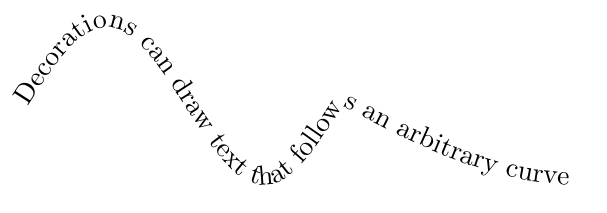
\begin{tikzpicture}
    \path [decorate,decoration={text along path,
        text={Decorations can draw text that follows an arbitrary curve}}]
        (0,0) sin (1,1) cos (2,0) sin (3,-1) cos (4,0) sin (7,-1);
\end{tikzpicture}

\begin{tikzpicture}[decoration={footprints,foot length=2pt}]
\draw decorate{ (0,0) -- (7,0)};
\end{tikzpicture}


\tikzset{paint/.style={ draw=#1!50!black, fill=#1!50 },
    decorate with/.style=
    {decorate,decoration={shape backgrounds,shape=#1,shape size=2mm}}}
\begin{tikzpicture}
\draw [decorate with=dart, paint=red] (0,1.5) to[bend left] (3,1.5);
\draw [decorate with=diamond, paint=green] (0,1) -- (3,1);
\draw [decorate with=rectangle, paint=blue,decoration={shape evenly spread=4}] (0,0.5) -- (3,0.5);
\draw [decorate with=star, paint=yellow] (0,0) to[bend right] (3,0);
\end{tikzpicture}

\end{document}


% What is new?

%%- New node shapes
%%
%%- Added overlay functionality to \node.
%%- Added pgfkeys and its documentation.
%%- Added fitting library.
%%
%%- \foreach will now allow a macro name to be given as list
%%      argument (as in \foreach \x in \mylist {...})
%%
%%- Added fadings.
%%    - Added functional shadings.
%%
%%- Added shadow library, removed shadow shapes (no longer
%%      needed).
%%    - Added preaction and postaction options (very useful).
%%    - Added transform canvas option.
%%    - Added scale around option.
%%
%%Coordinates like (2,3cm) are now allowed. Has the same
%%      effect as ([shift={(2,0)}]0pt,3cm), which is what everybody
%%      would expect.
%%
%%- Added decorations documentation.
%%Added calc library and ($...$) notation for coordinates
%%Added through library
%%Added tutorial for geometric constructions.
%%    - Fixed partway and intersection computations.
%%    - Added line to circle intersection.
%%
%%Finished chains and chain tutorial.
%%-positioning library

